\section{Résultats}

\subsection{Topics obtenus avec le NMF}
\subsubsection{Identification et interprétation des topics}

Une fois le modèle entraîné, les mots les plus importants de chaque topic ont été extraits afin de faciliter leur interprétation. Cette étape est essentielle, car le NMF ne produit pas directement des noms de thèmes : elle produit des groupes de mots. L'attribution d'un nom à chaque topic repose donc sur une analyse qualitative des termes les plus représentatifs.

Le tableau suivant présente les dix mots les plus caractéristiques de chaque topic obtenu avec la NMF. Ces mots servent de base à l'interprétation qualitative des thèmes extraits par le modèle.
\newpage

\begin{longtable}{p{1.8cm}p{11.5cm}}
\caption{Mots caractéristiques des topics obtenus avec la NMF} \\
\toprule
\textbf{Topic} & \textbf{Mots caractéristiques} \\
\midrule
\endfirsthead

\toprule
\textbf{Topic} & \textbf{Mots caractéristiques} \\
\midrule
\endhead
Topic 1 & femme, mari, chose, bon, homme, cher, ménage, histoire, vrai, plaisir \\
Topic 2 & travail, peuple, vie, usine, bonheur, justice, ouvrier, œuvre, humanité, terre \\
Topic 3 & arbre, soleil, herbe, eau, ciel, jardin, ombre, terre, feuille, branche \\
Topic 4 & million, bourse, cours, action, universelle, banque, affaire, agent, hausse, titre \\
Topic 5 & abbé, prêtre, curé, église, jardin, trouche, soutane, sous-préfecture, évêque \\
Topic 6 & table, verre, vin, pain, café, eau, maman, assiette, bon, petit \\
Topic 7 & main, œil, mort, bras, sang, tête, corps, face, voix, lèvre \\
Topic 8 & franc, argent, billet, somme, mois, sou, chiffre, pièce, fortune, poche \\
Topic 9 & monsieur, dame, porte, vou, bon, air, voix, tante, main, mot \\
Topic 10 & rue, maison, quartier, trottoir, boutique, boulevard, ville, place, voiture, chaussée \\
Topic 11 & train, gare, heure, machine, chef, voiture, voie, wagon, express, portière \\
Topic 12 & grotte, saint, sœur, malade, miracle, foule, cierge, foi, prêtre, pèlerin \\
Topic 13 & frère, sœur, modèle, petit, écriture, heure, pauvre, fine, lettre, témoin \\
Topic 14 & cardinal, pape, éminence, livre, palais, église, prêtre, don, prélat, romain \\
Topic 15 & école, instituteur, élève, vérité, église, classe, modèle, primaire, enseignement, juif \\
Topic 16 & père, fils, vieux, famille, fille, ferme, terre, paysan, maison, mort \\
Topic 17 & fosse, mineur, ouvrier, camarade, puits, coron, berline, galerie, porion, grève \\
Topic 18 & prussien, soldat, armée, général, route, cheval, corps, canon, capitaine, homme \\
Topic 19 & jeune, fille, homme, oncle, fine, nièce, garçon, mariage, tante, amant \\
Topic 20 & vendeur, rayon, magasin, comptoir, soie, dame, client, vente, bonheur, confection \\
Topic 21 & docteur, médecin, malade, maladie, visite, heure, jour, miracle, cher, jambe \\
Topic 22 & tableau, toile, peintre, peinture, œuvre, atelier, art, artiste, salle, étude \\
Topic 23 & chambre, lit, porte, heure, fenêtre, nuit, escalier, pièce, maison, meuble \\
Topic 24 & enfant, mère, petit, fille, maman, pauvre, nourrice, bon, larme, œil \\
Topic 25 & bel, halle, charcuterie, quenu, boutique, gras, charcutier, marchand, normande, blanc \\
Topic 26 & salon, comte, dame, comtesse, satin, marquis, blanc, rose, femme, petit \\
Topic 27 & empereur, ministre, député, préfet, président, colonel, politique, affaire, lettre, ami \\
Topic 28 & amour, cœur, vie, tendresse, jour, pensée, bonheur, amant, heure, joie \\
Topic 29 & insurgé, barricade, national, ville, fusil, garde, républicain, ouvrier, place, peuple \\
\bottomrule
\end{longtable}

Chaque topic a ensuite été nommé à partir des mots dominants et de l'observation des segments les plus fortement associés à ce topic. Cette double vérification permet de limiter les erreurs d'interprétation. En effet, certains mots peuvent sembler cohérents isolément, mais prendre un sens différent lorsqu'ils sont replacés dans les extraits du corpus.

Les topics obtenus couvrent plusieurs dimensions importantes de l'œuvre de Zola. Certains renvoient à des espaces sociaux précis, comme le magasin, la mine, la bourse, le quartier ou le monde ferroviaire. D'autres correspondent à des thèmes plus transversaux, comme la famille, le désir, la maladie, la religion, la pauvreté ou la mort. Cette diversité montre que le NMF permet de faire apparaître à la fois des thèmes sociaux, des motifs narratifs et des univers propres à certains romans.

\subsubsection{Nommer les topics}

Les topics ont ensuite été nommés manuellement à partir des mots les plus représentatifs et des segments les plus fortement associés. Cette étape constitue une part qualitative importante de l'analyse. Elle permet de transformer les résultats numériques du modèle en catégories interprétables.
\newpage 

\begin{longtable}{p{2cm}p{11cm}}
\caption{Noms attribués aux topics obtenus avec la NMF} \\
\toprule
\textbf{Topic} & \textbf{Nom attribué} \\
\midrule
\endfirsthead

\toprule
\textbf{Topic} & \textbf{Nom attribué} \\
\midrule
\endhead

Topic 1 & Les relations conjugales et la vie domestique \\
Topic 2 & Le travail, le peuple et la justice sociale \\
Topic 3 & La nature et le paysage \\
Topic 4 & La bourse, la finance et les affaires \\
Topic 5 & Le clergé et la paroisse \\
Topic 6 & La table et les repas \\
Topic 7 & Le corps, la souffrance et la mort \\
Topic 8 & L'argent et la fortune \\
Topic 9 & Les conversations et les scènes domestiques \\
Topic 10 & Le quartier et la ville \\
Topic 11 & Le monde ferroviaire \\
Topic 12 & Le miracle, le pèlerinage et la religion \\
Topic 13 & Les liens familiaux, l'écriture et les proches \\
Topic 14 & Le pouvoir religieux \\
Topic 15 & L'école et l'instruction \\
Topic 16 & La famille, la terre et le monde paysan \\
Topic 17 & Le monde ouvrier et la mine \\
Topic 18 & La guerre, les soldats et l'armée \\
Topic 19 & Le désir, le mariage et les relations amoureuses \\
Topic 20 & Le magasin, la vente et les clientes \\
Topic 21 & Le monde médical et la santé \\
Topic 22 & Le monde artistique et la peinture \\
Topic 23 & La chambre, le lit et l'espace intime \\
Topic 24 & L'enfance, la maternité et la pauvreté \\
Topic 25 & Le commerce alimentaire et les halles \\
Topic 26 & Le salon, l'aristocratie et les scènes mondaines \\
Topic 27 & Le pouvoir politique et les affaires publiques \\
Topic 28 & L'amour, le bonheur et les sentiments \\
Topic 29 & L'insurrection et la révolution \\

\bottomrule
\end{longtable}

Cette étape montre que l’analyse ne repose pas uniquement sur une extraction automatique. Le modèle propose des regroupements de mots, mais leur interprétation dépend d’un travail humain. Les noms attribués aux topics doivent donc être compris comme des catégories d’analyse construites à partir des résultats du modèle, et non comme des vérités objectives produites automatiquement par l’algorithme.

\subsection{Nombre de segments associés à chaque topic dominant}

Afin d'analyser la répartition des thèmes dans le corpus, un topic dominant a été attribué à chaque segment. Pour cela, les poids de la matrice \texttt{W} ont d'abord été normalisés afin de rendre les contributions des topics comparables entre les segments. Le topic dominant correspond ensuite au topic dont le poids est le plus élevé pour un segment donné.

La colonne \texttt{topic\_dominant} indique donc le topic le plus représenté dans chaque paquet de phrases. La colonne \texttt{poids\_topic} mesure l'intensité de cette association : plus cette valeur est élevée, plus le segment est clairement associé à un topic spécifique. À l'inverse, un poids faible peut signaler un segment plus mixte, contenant plusieurs thèmes ou ne correspondant fortement à aucun topic.

Cette attribution permet de passer d'une simple liste de topics à une analyse plus structurée de leur répartition dans le corpus. Elle rend possible l'étude du nombre de segments associés à chaque topic, du poids moyen des topics dans l'ensemble du corpus et de leur présence selon les romans. Le tableau suivant présente le nombre de segments associés à chaque topic dominant.

\begin{longtable}{p{10cm}r}
\caption{Nombre de segments associés à chaque topic dominant} \\
\toprule
\textbf{Topic dominant} & \textbf{Nombre de segments} \\
\midrule
\endfirsthead

\toprule
\textbf{Topic dominant} & \textbf{Nombre de segments} \\
\midrule
\endhead
L'amour, le bonheur et les sentiments & 335 \\
La chambre, le lit et l'espace intime & 327 \\
Le pouvoir politique et les affaires publiques & 266 \\
Le salon, l'aristocratie et les scènes mondaines & 266 \\
Le travail, le peuple et la justice sociale & 262 \\
La nature et le paysage & 229 \\
L'enfance, la maternité et la pauvreté & 221 \\
Le corps, la souffrance et la mort & 218 \\
La table et les repas & 214 \\
Le clergé et la paroisse & 210 \\
Le quartier et la ville & 205 \\
L'argent et la fortune & 187 \\
Le monde ouvrier et la mine & 185 \\
La famille, la terre et le monde paysan & 180 \\
Le miracle, le pèlerinage et la religion & 177 \\
Le désir, le mariage et les relations amoureuses & 173 \\
La guerre, les soldats et l'armée & 173 \\
L'école et l'instruction & 168 \\
Le monde médical et la santé & 164 \\
Le commerce alimentaire et les halles & 163 \\
Les conversations et les scènes domestiques & 162 \\
Le monde artistique et la peinture & 141 \\
Le pouvoir religieux & 140 \\
Le magasin, la vente et les clientes & 136 \\
L'insurrection et la révolution & 127 \\
Les liens familiaux, l'écriture et les proches & 104 \\
Le monde ferroviaire & 94 \\
La bourse, la finance et les affaires & 69 \\
Les relations conjugales et la vie domestique & 31 \\
\bottomrule
\end{longtable}

La répartition des segments montre que les topics ne sont pas représentés de manière parfaitement équilibrée. Certains thèmes regroupent un nombre important de segments, tandis que d'autres apparaissent de façon plus marginale. Cette variation est attendue dans un corpus littéraire, car tous les motifs thématiques ne sont pas présents avec la même intensité dans l'ensemble des romans.

Les topics les plus représentés correspondent aux thèmes qui structurent fortement le corpus. Les premiers résultats font apparaître des motifs liés aux sentiments, à l'espace intime, aux relations sociales, au pouvoir politique, aux scènes mondaines ou encore au travail. Ces ensembles renvoient à des dimensions récurrentes de l'œuvre de Zola, dans laquelle les expériences individuelles sont souvent articulées à des milieux sociaux, familiaux, économiques ou institutionnels.

À l'inverse, les topics les moins représentés ne doivent pas être considérés comme moins importants sur le plan littéraire. Ils peuvent correspondre à des univers plus localisés, associés à certains romans précis ou à des situations narratives particulières. C'est notamment le cas de thèmes comme la bourse, le monde ferroviaire ou certaines formes de relations domestiques, qui peuvent être fortement présents dans quelques œuvres sans être répartis de manière uniforme dans l'ensemble du corpus.

Cette distribution montre donc que la NMF ne produit pas seulement une liste de thèmes interprétables : elle permet aussi d'évaluer leur poids relatif dans le corpus. Le nombre de segments associés à chaque topic donne une première indication de l'importance quantitative des thèmes extraits. Cette mesure doit toutefois être interprétée avec prudence : un topic fréquent n'est pas nécessairement plus important sur le plan littéraire, mais il est plus présent lexicalement dans les segments analysés.

Enfin, cette attribution des topics dominants peut servir de base à des analyses complémentaires. Elle permet notamment d'étudier la distribution des topics par œuvre, de comparer les romans entre eux, ou encore d'appliquer ultérieurement un détecteur de motifs aux segments associés à chaque topic afin d'identifier les motifs narratifs les plus caractéristiques de chaque thème.

\subsection{Clusters obtenus avec K-means}

\subsubsection{Extraction des mots caractéristiques des clusters}

Une fois le modèle entraîné, les centres des clusters ont été analysés afin d'identifier les termes les plus représentatifs de chaque groupe. Dans K-means, chaque cluster est représenté par un centroïde, c'est-à-dire un point moyen dans l'espace vectoriel. Les termes les plus fortement associés à ce centroïde permettent de comprendre le contenu thématique du cluster.

Cette étape est comparable à l'extraction des mots dominants dans la NMF. Elle permet d'associer chaque cluster à un ensemble de termes caractéristiques. Cependant, l'interprétation est légèrement différente : dans la NMF, les mots sont associés à un topic latent ; dans K-means, ils décrivent le centre lexical d'un groupe de segments. Autrement dit, les mots obtenus indiquent ce qui rapproche les segments d'un même cluster.

\begin{longtable}{p{2cm}p{11.5cm}}
\caption{Mots caractéristiques des clusters obtenus avec K-means} \\
\toprule
\textbf{Cluster} & \textbf{Mots caractéristiques} \\
\midrule
\endfirsthead

\toprule
\textbf{Cluster} & \textbf{Mots caractéristiques} \\
\midrule
\endhead
Cluster 1 & verre, petit, table, maman, coup, femme, vin, eau, tête, homme \\
Cluster 2 & instituteur, école, enfant, vérité, élève, petit, église, père, classe, bon \\
Cluster 3 & salon, dame, femme, monsieur, petit, blanc, satin, homme, jeune, rose \\
Cluster 4 & chambre, porte, lit, monsieur, heure, femme, petit, maison, escalier, fenêtre \\
Cluster 5 & enfant, femme, nourrice, petit, usine, constance, fille, mari, monsieur, cher \\
Cluster 6 & mère, fille, petit, enfant, père, femme, fils, bon, jeune, œil \\
Cluster 7 & train, gare, chef, machine, voie, heure, express, mécanicien, tunnel, voyageur \\
Cluster 8 & amour, cœur, vie, jeune, enfant, femme, fille, jour, homme, tendresse \\
Cluster 9 & comte, comtesse, monsieur, scène, loge, femme, prullière, homme, théâtre, dame \\
Cluster 10 & abbé, prêtre, curé, monsieur, église, bon, tête, petit, frère, enfant \\
Cluster 11 & arbre, soleil, herbe, ciel, eau, ombre, jardin, blanc, haut, terre \\
Cluster 12 & grotte, saint, miracle, cierge, prêtre, malade, foule, foi, père, église \\
Cluster 13 & docteur, médecin, monsieur, enfant, mère, petit, malade, heure, œil, lit \\
Cluster 14 & sœur, malade, hyacinthe, wagon, saint, train, petit, compartiment, pèlerin, grotte \\
Cluster 15 & insurgé, ville, national, fusil, barricade, républicain, homme, garde, ouvrier, rue \\
Cluster 16 & rue, boutique, trottoir, petit, quartier, maison, femme, bel, halle, heure \\
Cluster 17 & femme, jeune, amant, chambre, main, pensée, œil, bras, nuit, homme \\
Cluster 18 & empereur, ministre, monsieur, député, colonel, homme, affaire, préfet, gouvernement, ami \\
Cluster 19 & travail, vie, enfant, terre, petit, usine, ouvrier, peuple, œuvre, homme \\
Cluster 20 & bourse, million, franc, action, cours, banque, universelle, monsieur, hausse, argent \\
Cluster 21 & franc, argent, monsieur, femme, homme, jeune, jour, billet, somme, bon \\
Cluster 22 & monsieur, dame, femme, petit, porte, bon, fille, air, homme, chambre \\
Cluster 23 & tableau, peintre, toile, peinture, œuvre, art, atelier, femme, artiste, salon \\
Cluster 24 & fosse, mineur, coron, camarade, berline, homme, ouvrier, puits, grève, porion \\
Cluster 25 & vendeur, rayon, magasin, comptoir, dame, soie, vente, client, bonheur, franc \\
Cluster 26 & prussien, soldat, armée, général, route, homme, cheval, capitaine, corps, canon \\
Cluster 27 & cardinal, pape, palais, éminence, livre, prêtre, monde, église, peuple, prélat \\
Cluster 28 & frère, modèle, petit, père, vérité, président, homme, crime, justice, écriture \\
Cluster 29 & père, terre, vieux, petit, coup, bon, vache, homme, paysan, bête \\
\bottomrule
\end{longtable}

Cette extraction permet de vérifier la cohérence interne des clusters. Lorsqu'un cluster rassemble des mots appartenant au même champ lexical, il devient plus facilement interprétable. À l'inverse, un cluster contenant des mots trop dispersés ou peu cohérents peut indiquer un regroupement moins stable ou plus difficile à nommer.

\subsubsection{Nomination des clusters}

Les clusters ont ensuite été nommés manuellement à partir des mots les plus représentatifs et de l'observation des segments associés. Cette étape est indispensable, car K-means ne produit pas directement des intitulés interprétables. Comme pour la NMF, le passage du résultat numérique à l'interprétation thématique repose donc sur une lecture qualitative et est lié a l'interprétation humaine (chaque noms de clusters peut donc etre remis en cause).

\begin{longtable}{p{2cm}p{11cm}}
\caption{Noms attribués aux clusters obtenus avec K-means} \\
\toprule
\textbf{Cluster} & \textbf{Nom attribué} \\
\midrule
\endfirsthead

\toprule
\textbf{Cluster} & \textbf{Nom attribué} \\
\midrule
\endhead
Cluster 1 & La table, les repas et les boissons \\
Cluster 2 & L'école, les élèves et l'instruction \\
Cluster 3 & Le salon, l'aristocratie et les apparences \\
Cluster 4 & La chambre, le lit et l'espace domestique \\
Cluster 5 & L'enfance, la maternité et la pauvreté \\
Cluster 6 & La mère, les enfants et la famille \\
Cluster 7 & Le monde ferroviaire \\
Cluster 8 & L'amour, les sentiments et la jeunesse \\
Cluster 9 & Le théâtre, la loge et les scènes mondaines \\
Cluster 10 & Le clergé et la paroisse \\
Cluster 11 & La nature et le paysage \\
Cluster 12 & Le miracle, le pèlerinage et la religion \\
Cluster 13 & Le monde médical et la santé \\
Cluster 14 & Le pèlerinage, la maladie et le voyage \\
Cluster 15 & L'insurrection et la révolution \\
Cluster 16 & Le quartier, la rue et la ville \\
Cluster 17 & Le désir, le corps et les relations amoureuses \\
Cluster 18 & Le pouvoir politique et les affaires publiques \\
Cluster 19 & Le travail, le peuple et le monde ouvrier \\
Cluster 20 & La bourse, la finance et les affaires \\
Cluster 21 & L'argent du quotidien \\
Cluster 22 & Les conversations et les scènes domestiques \\
Cluster 23 & Le monde artistique et la peinture \\
Cluster 24 & La mine, les ouvriers et la grève \\
Cluster 25 & Le magasin, la vente et les clientes \\
Cluster 26 & La guerre, les soldats et l'armée \\
Cluster 27 & Le pouvoir religieux \\
Cluster 28 & Les liens familiaux, l'écriture et la justice \\
Cluster 29 & La terre, les animaux et le monde paysan \\
\bottomrule
\end{longtable}

Les intitulés obtenus montrent que les clusters couvrent des dimensions proches de celles observées avec la NMF. On retrouve par exemple des ensembles liés au travail, à la mine, à la finance, à la religion, à la famille, au monde domestique, à la guerre ou encore aux espaces urbains.

Cependant, les clusters K-means ne doivent pas être interprétés comme des catégories fixes ou naturelles. Ils résultent d'un regroupement algorithmique fondé sur la proximité lexicale des segments. Leur nomination repose donc sur un choix interprétatif, à partir des mots les plus représentatifs et des extraits textuels associés.

\subsubsection{Regroupement hiérarchique des clusters}

Afin de compléter l’analyse des clusters obtenus avec K-means, une classification ascendante hiérarchique a été appliquée aux centroïdes des 29 clusters. Cette étape permet d’examiner les proximités entre clusters et de regrouper ceux qui présentent des profils lexicaux similaires. Elle offre ainsi une lecture plus synthétique de la structure thématique du corpus, en passant d’une analyse détaillée cluster par cluster à une organisation en grandes familles de motifs.

La méthode de Ward a été retenue pour construire cette hiérarchie. Elle consiste à fusionner progressivement les clusters en minimisant l’augmentation de la variance interne à chaque regroupement. Le dendrogramme obtenu permet de visualiser les distances entre clusters et d’identifier les principaux rapprochements thématiques\footnote{Ludovic Lebart et André Salem, \textit{Statistique textuelle}, Paris, Dunod, 1994.}.

\begin{figure}[H]
    \centering
    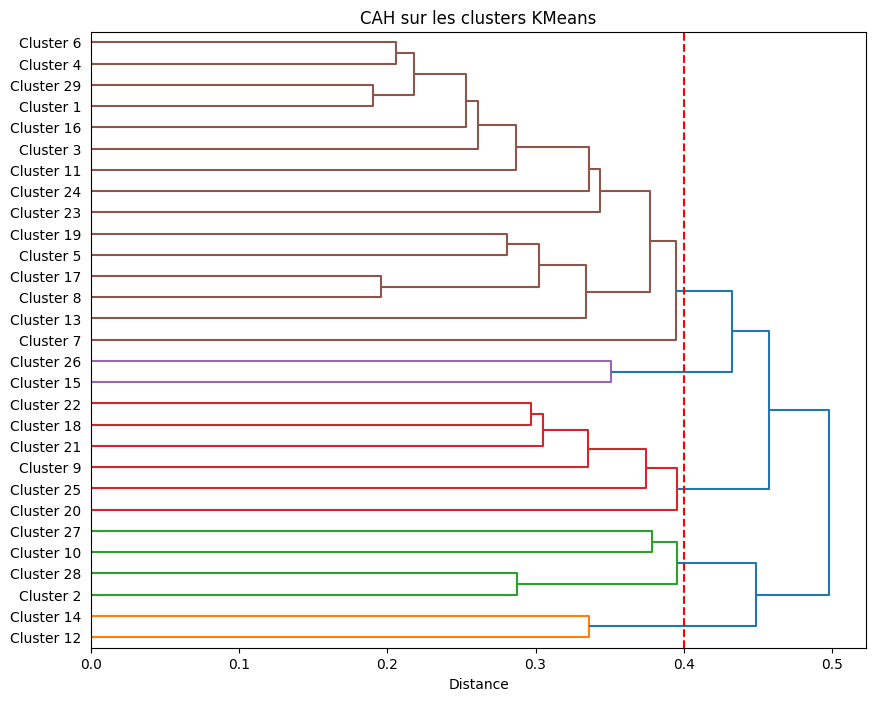
\includegraphics[width=\textwidth]{images/chapitre_1/resultats/dendrogramme.png}
    \caption{Dendrogramme de la classification hiérarchique des clusters K-means}
    \label{fig:dendrogramme}
\end{figure}

Dans cette analyse, le seuil de distance a été fixé à 0,40 afin de découper l’arbre hiérarchique en grandes familles de motifs. Ce regroupement rend les résultats plus lisibles : les 29 clusters initiaux peuvent être interprétés non seulement individuellement, mais aussi comme des ensembles thématiques plus larges. Cette organisation facilite ensuite la comparaison entre les motifs dominants du corpus et leur répartition dans les romans de Zola.

\subsubsection{Création des grandes familles de motifs}

À partir du dendrogramme, les clusters ont été regroupés en cinq grandes familles de motifs. Cette opération permet de simplifier l'analyse et de faire apparaître les grandes zones thématiques du corpus.

\begin{figure}[H]
    \centering
    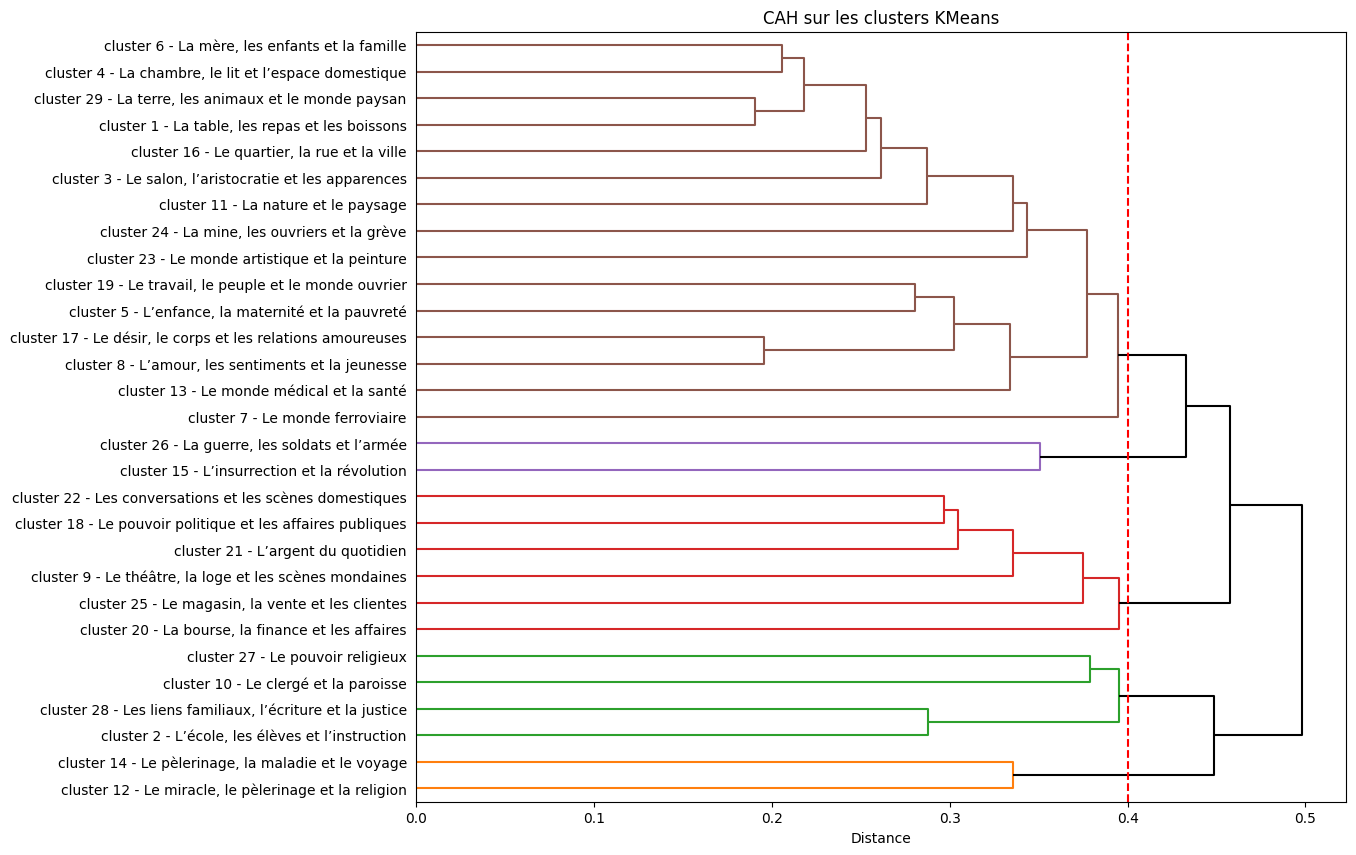
\includegraphics[width=\textwidth,height=18cm,keepaspectratio]{images/chapitre_1/resultats/dendrogramme_clusters.png}
    \caption{Regroupement des clusters K-means en grandes familles de motifs}
    \label{fig:groupes_cah}
\end{figure}

Les groupes obtenus ont ensuite été nommés manuellement, en fonction des clusters qu'ils rassemblent. Le tableau suivant présente la composition de chaque grande famille de motifs.
\newpage
\begin{longtable}{p{2cm}p{11.5cm}}
\caption{Composition des grandes familles de motifs issues des clusters K-means} \\
\toprule
\textbf{Groupe} & \textbf{Clusters associés} \\
\midrule
\endfirsthead

\toprule
\textbf{Groupe} & \textbf{Clusters associés} \\
\midrule
\endhead

Groupe 1 & 
Cluster 12 : Le miracle, le pèlerinage et la religion ; 
Cluster 14 : Le pèlerinage, la maladie et le voyage. \\

Groupe 2 & 
Cluster 2 : L'école, les élèves et l'instruction ; 
Cluster 10 : Le clergé et la paroisse ; 
Cluster 27 : Le pouvoir religieux ; 
Cluster 28 : Les liens familiaux, l'écriture et la justice. \\

Groupe 3 & 
Cluster 9 : Le théâtre, la loge et les scènes mondaines ; 
Cluster 18 : Le pouvoir politique et les affaires publiques ; 
Cluster 20 : La bourse, la finance et les affaires ; 
Cluster 21 : L'argent du quotidien ; 
Cluster 22 : Les conversations et les scènes domestiques ; 
Cluster 25 : Le magasin, la vente et les clientes. \\

Groupe 4 & 
Cluster 15 : L'insurrection et la révolution ; 
Cluster 26 : La guerre, les soldats et l'armée. \\

Groupe 5 & 
Cluster 1 : La table, les repas et les boissons ; 
Cluster 3 : Le salon, l'aristocratie et les apparences ; 
Cluster 4 : La chambre, le lit et l'espace domestique ; 
Cluster 5 : L'enfance, la maternité et la pauvreté ; 
Cluster 6 : La mère, les enfants et la famille ; 
Cluster 7 : Le monde ferroviaire ; 
Cluster 8 : L'amour, les sentiments et la jeunesse ; 
Cluster 11 : La nature et le paysage ; 
Cluster 13 : Le monde médical et la santé ; 
Cluster 16 : Le quartier, la rue et la ville ; 
Cluster 17 : Le désir, le corps et les relations amoureuses ; 
Cluster 19 : Le travail, le peuple et le monde ouvrier ; 
Cluster 23 : Le monde artistique et la peinture ; 
Cluster 24 : La mine, les ouvriers et la grève ; 
Cluster 29 : La terre, les animaux et le monde paysan. \\

\bottomrule
\end{longtable}

Ces grandes familles permettent d'obtenir une lecture plus synthétique des résultats. La première famille regroupe les motifs liés au miracle, au pèlerinage et à la religion. La deuxième rassemble des clusters associés aux formes d'encadrement social, religieux, scolaire et familial. La troisième renvoie davantage aux espaces sociaux, économiques et mondains, en regroupant notamment la finance, le commerce, le théâtre et les conversations domestiques. La quatrième famille réunit les motifs du conflit collectif, de l'insurrection et de la guerre. Enfin, la cinquième regroupe un ensemble plus large de motifs liés à la vie quotidienne, aux espaces sociaux, au travail, à la famille, à la nature et aux expériences individuelles.

Cette structuration est particulièrement utile pour l'analyse littéraire, car elle permet de passer d'une liste de clusters nombreux à une organisation thématique plus lisible. Elle montre aussi que les motifs extraits par K-means ne sont pas isolés, mais peuvent être regroupés en ensembles plus larges correspondant à des dimensions importantes de l'œuvre de Zola.

\subsubsection{Attribution des grandes familles aux segments}

Une fois les groupes hiérarchiques définis, chaque segment du corpus a reçu une étiquette correspondant à la grande famille de motifs associée à son cluster\footnote{Voir code en annexe}. Cette opération permet d'analyser non seulement les clusters détaillés, mais aussi les grandes catégories thématiques dans lesquelles ils s'inscrivent.

\begin{figure}[H]
    \centering
    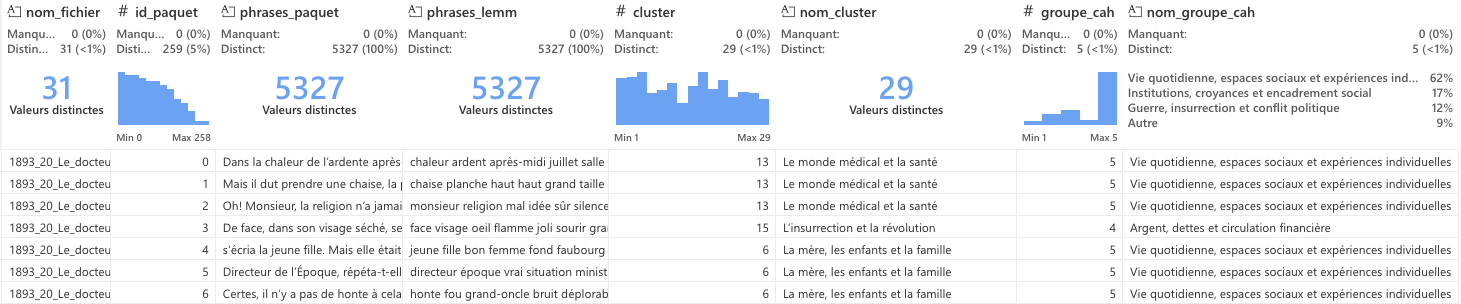
\includegraphics[width=\textwidth]{images/chapitre_1/resultats/df_annote.png}
    \caption{Noms attribués aux grandes familles de motifs}
    \label{fig:noms_groupes_cah}
\end{figure}

Cette étape permet de relier chaque paquet de phrases à deux niveaux d'analyse. Le premier niveau est le cluster K-means, qui fournit une catégorie thématique fine. Le second niveau est le groupe CAH, qui fournit une catégorie plus générale. Cette double échelle d'interprétation est utile, car elle permet d'adapter le niveau de détail selon les besoins de l'analyse : on peut étudier les motifs précis, ou bien observer les grandes tendances du corpus.

\subsubsection{Analyse de la répartition des clusters}

Après la nomination des clusters et des grandes familles, plusieurs visualisations ont été produites afin d'étudier leur répartition dans le corpus. La première consiste à compter le nombre de segments associés à chaque grande famille de motifs.

\begin{figure}[H]
    \centering
    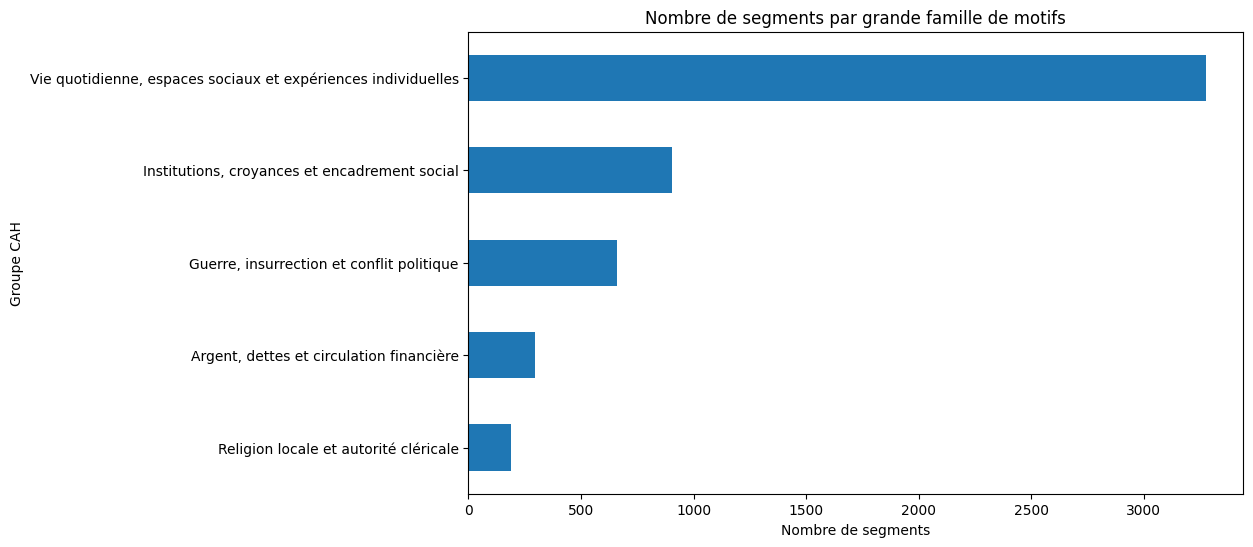
\includegraphics[width=\textwidth]{images/chapitre_1/resultats/nb_segment_famille_cluster.png}
    \caption{Distribution des grandes familles de motifs dans le corpus}
    \label{fig:distribution_groupes_cah}
\end{figure}

Cette visualisation permet d'identifier les grandes familles les plus représentées dans l'ensemble du corpus. Elle donne une lecture globale de l'organisation thématique des segments. Une famille très représentée indique qu'un ensemble de motifs revient fréquemment dans les romans, tandis qu'une famille moins présente peut correspondre à un thème plus spécifique, associé à certains romans ou à certaines situations narratives.

Une seconde visualisation a été produite à l'échelle des clusters détaillés.

\begin{figure}[H]
    \centering
    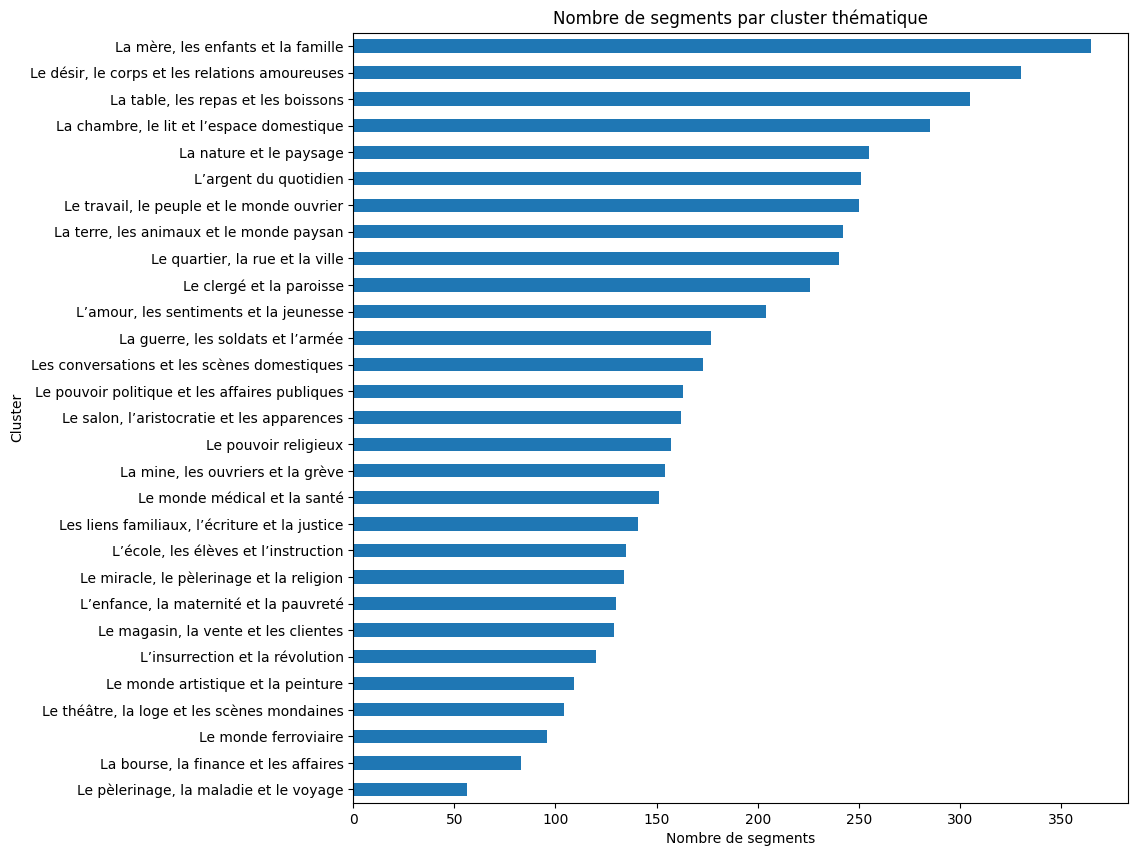
\includegraphics[width=\textwidth]{images/chapitre_1/resultats/nb_segment_cluster.png}
    \caption{Distribution des clusters K-means dans le corpus}
    \label{fig:distribution_clusters_kmeans}
\end{figure}

Cette représentation permet de voir quels clusters sont les plus fréquents dans le corpus. Elle est plus précise que l'analyse par grandes familles, car elle distingue les motifs thématiques particuliers. Elle permet par exemple d'observer séparément les clusters associés à la mine, à la finance, à la religion, à la famille ou au monde domestique.

